\section{Lab 2: Triển khai Mô hình Mạng 3 Lớp Truyền Thống (Hierarchical L3)}

\subsection{Kiến trúc Tổng quan và Phân bổ Tài nguyên}
Khắc phục nhược điểm của mạng phẳng, Mô hình 2 áp dụng kiến trúc phân cấp 3 lớp tiêu chuẩn: Core - Distribution - Access. Hệ thống sử dụng VLAN để cô lập các miền quảng bá (Broadcast Domain) và kích hoạt giao thức STP (Spanning Tree Protocol) trên toàn bộ Switch để chống lặp vòng (Loop).

\begin{figure}[H]
    \centering
    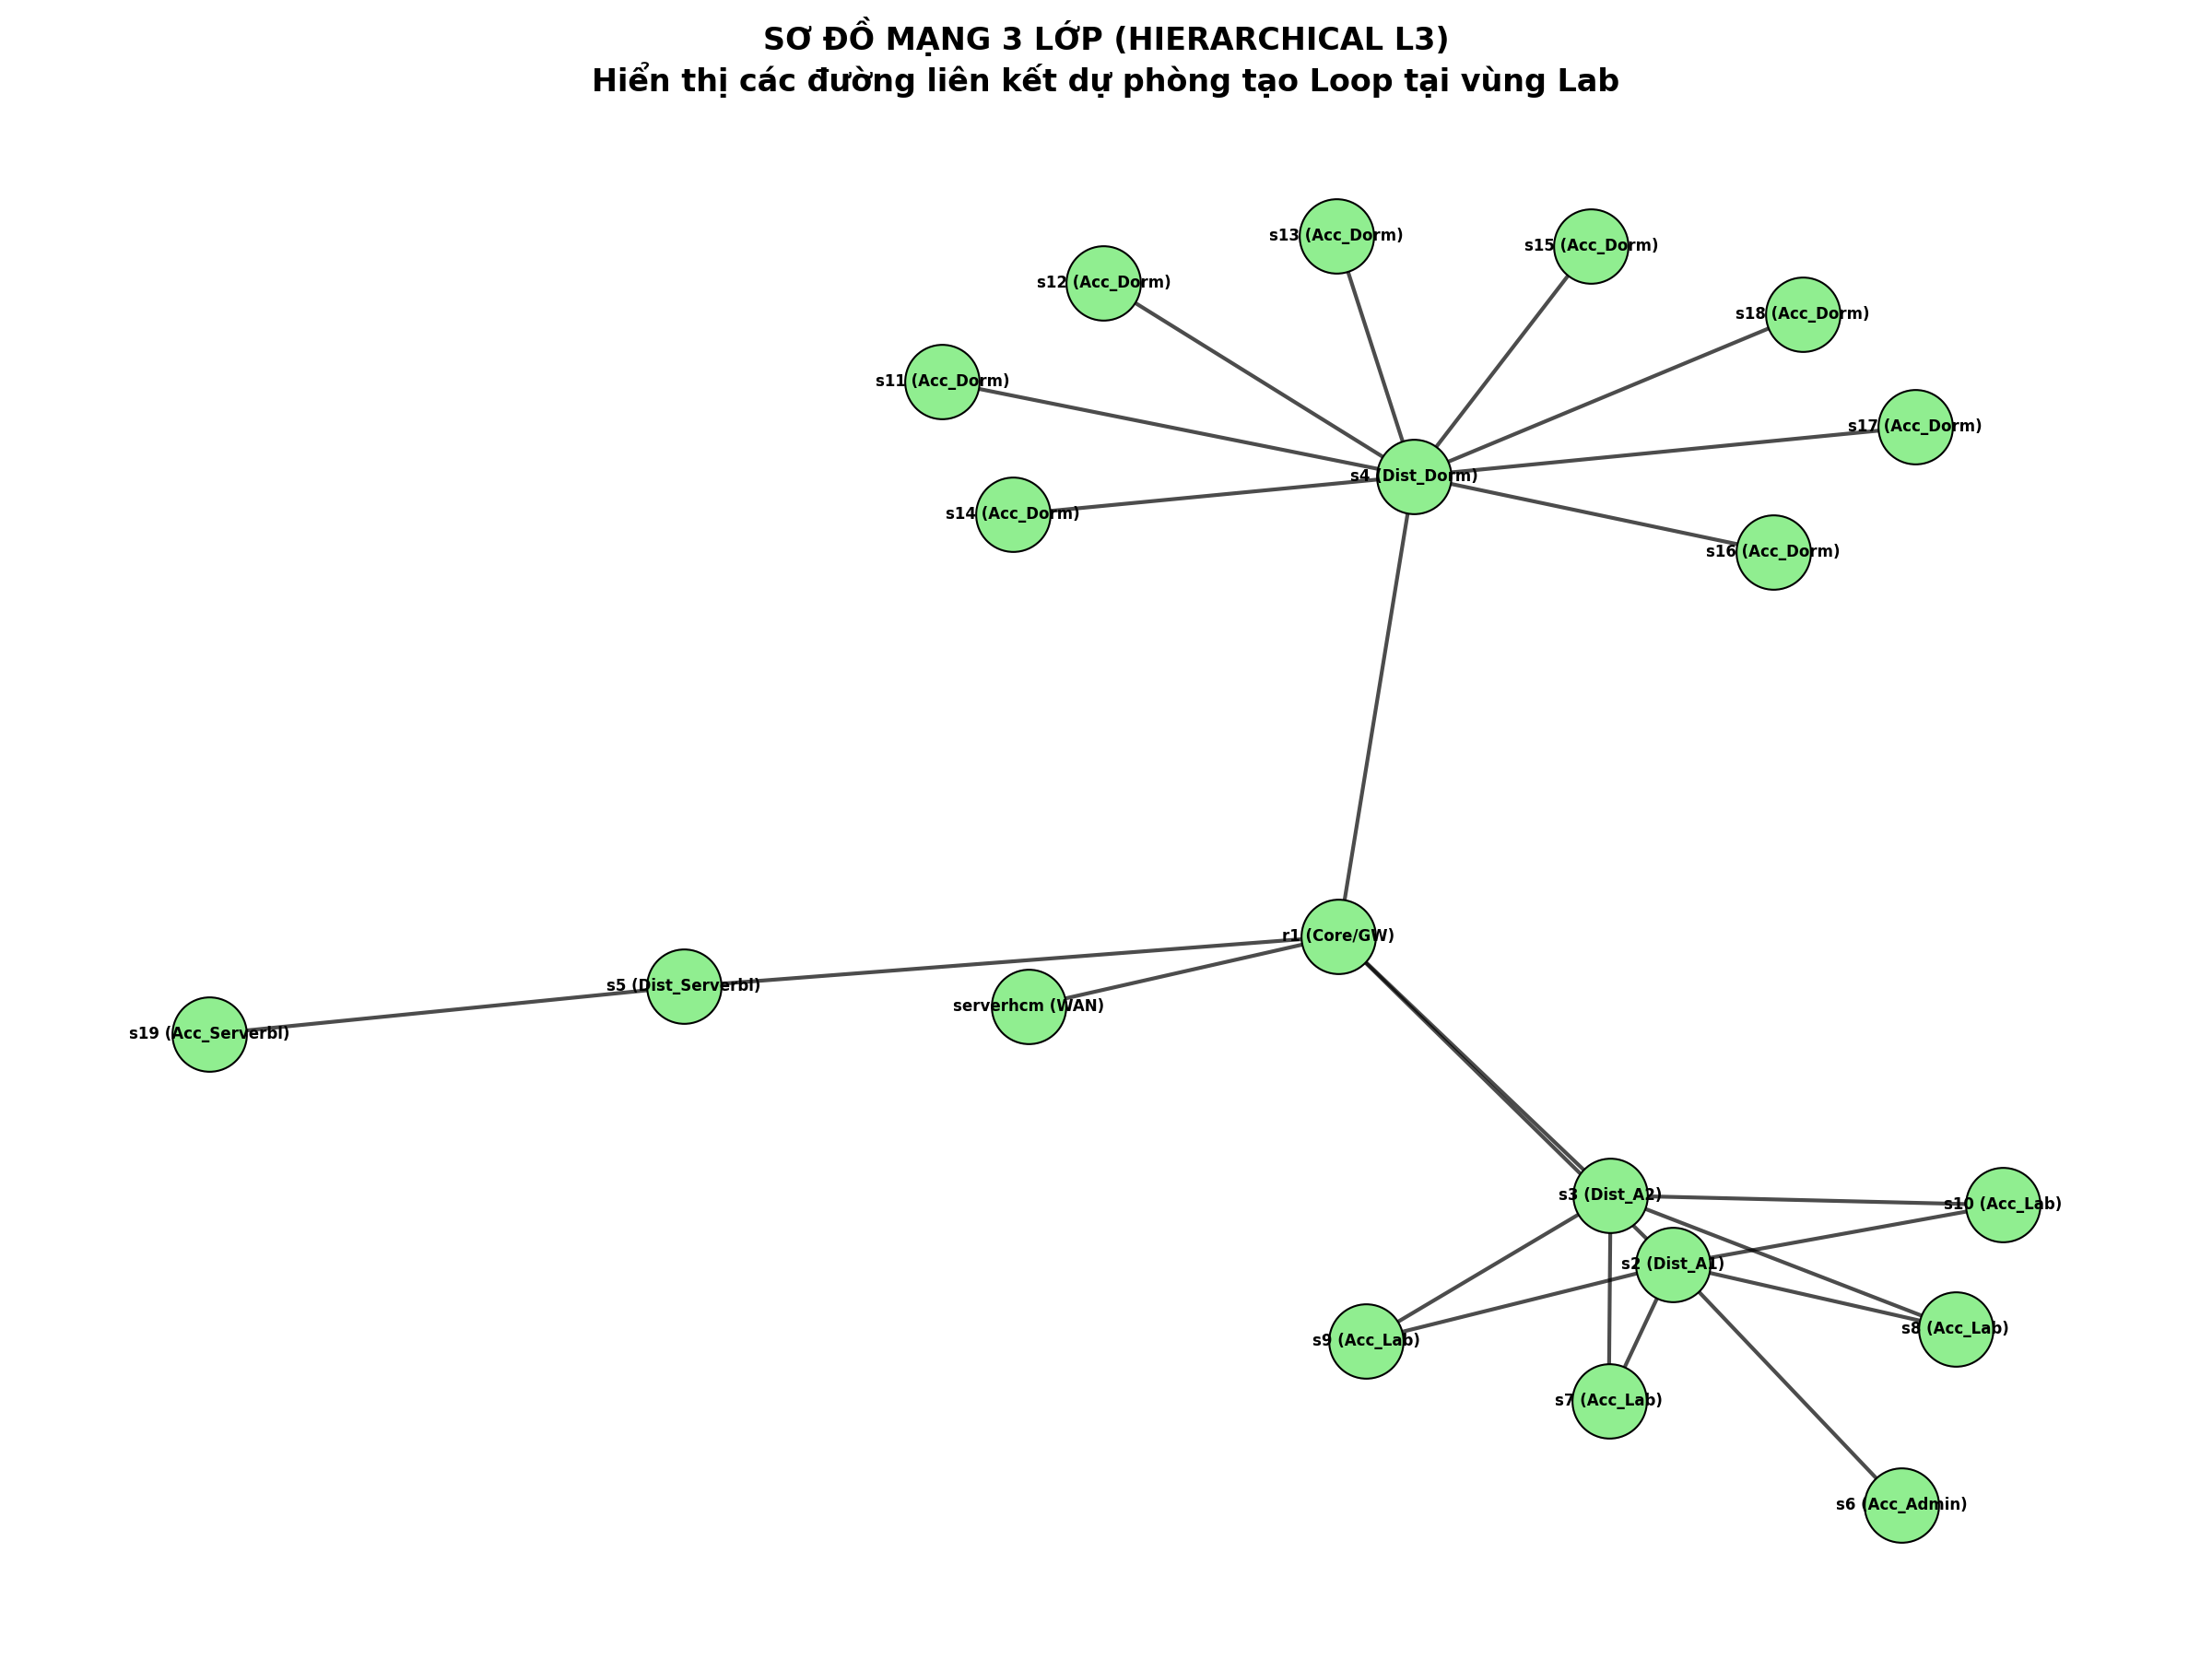
\includegraphics[width=0.8\linewidth]{image/topology_mohinh2.png}
    \caption{Sơ đồ kiến trúc mạng 3 lớp (Hierarchical L3) với các liên kết dự phòng}
    \label{fig:mh2_topo}
\end{figure}

\subsection{Quy hoạch Không gian IP và VLAN}
Mạng nội bộ được chia thành 4 VLAN riêng biệt với các Gateway tương ứng cấu hình trên Core Router (\texttt{r1}):
\begin{itemize}
    \item \textbf{VLAN 10 (Admin):} Dải IP \texttt{10.0.10.0/24}, Gateway: \texttt{10.0.10.254}
    \item \textbf{VLAN 20 (Lab AI):} Dải IP \texttt{10.0.20.0/24}, Gateway: \texttt{10.0.20.254}
    \item \textbf{VLAN 30 (Dorm):} Dải IP \texttt{10.0.30.0/24}, Gateway: \texttt{10.0.30.254}
    \item \textbf{VLAN 99 (Server Local):} Dải IP \texttt{10.0.99.0/24}, Gateway: \texttt{10.0.99.254}
\end{itemize}

\subsection{Thao tác Thực thi trong Môi trường Ubuntu Linux}

\subsubsection{Khởi chạy và Chờ Hội tụ STP}
\begin{lstlisting}[language=bash]
# Xoa mo hinh cu va khoi chay kich ban
sudo mn -c
sudo python3 cauhinh2.py
\end{lstlisting}
Khác với mạng phẳng, sau khi khởi động, hệ thống cần khoảng 20 giây để giao thức STP tính toán cây khung, bầu chọn Root Bridge và chuyển các cổng dự phòng sang trạng thái Block/Discarding để chống Loop.

\begin{figure}[H]
    \centering
    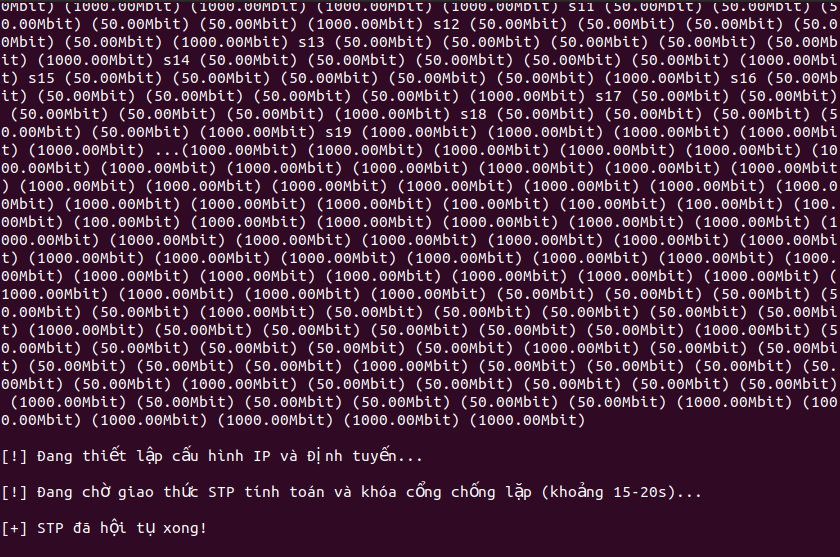
\includegraphics[width=0.8\linewidth]{image/stp_convergence.png}
    \caption{Quá trình chờ STP hội tụ và khóa cổng trên giao diện dòng lệnh}
    \label{fig:stp_convergence}
\end{figure}

\subsection{Các Kịch bản Kiểm thử Hiệu năng}

\subsubsection{Bài Test 1: Kiểm tra Định tuyến Inter-VLAN}
Mục đích: Xác nhận Core Router đã định tuyến thành công giữa các VLAN bị cô lập.
\begin{lstlisting}[language=bash]
# Tu vung Admin (VLAN 10) ping den Server (VLAN 99)
mininet> admin1 ping -c 4 10.0.99.1
\end{lstlisting}

\subsubsection{Bài Test 2: Băng thông East-West \& Sự lãng phí của STP}
Mục đích: Chứng minh STP làm lãng phí băng thông dự phòng. Dù Lab có nhiều đường link 1Gbps nối lên Distribution, STP đã khóa một nửa số đường này. Lưu lượng từ Lab dồn vào một Uplink duy nhất.
\begin{lstlisting}[language=bash]
# Mo iperf server tren serverbl1
mininet> serverbl1 iperf -s &

# Day luong du lieu lon (Elephant Flow) tu lab1
mininet> lab1 iperf -c 10.0.99.1 -t 10

# Kiem tra cong bi khoa boi STP tren Switch
mininet> sh ovs-ofctl show s7
\end{lstlisting}
\textbf{Đánh giá kết quả:} Tổng băng thông đo được bị giới hạn cứng ở mức 1Gbps của đường Uplink đang Active. Các đường link dự phòng hoàn toàn không được sử dụng để chia sẻ tải.

\begin{figure}[H]
    \centering
    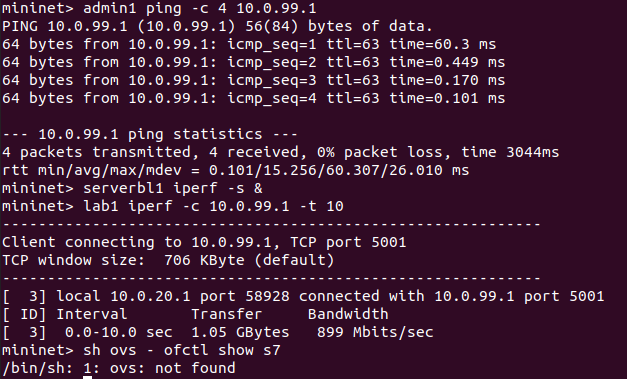
\includegraphics[width=0.8\linewidth]{image/iperf_test2.png}
    \caption{Băng thông tối đa bị kẹt ở mức 1Gbps do STP khóa cổng dự phòng}
    \label{fig:iperf_test2}
\end{figure}

\subsubsection{Bài Test 3: Nghẽn mạng WAN (Oversubscription)}
Mục đích: Đánh giá khả năng kiểm soát luồng.
\begin{lstlisting}[language=bash]
# Tao traffic UDP 250Mbps tu Dorm day ra WAN
mininet> dorm1 iperf -c 203.162.1.1 -u -b 250M -t 15 &

# Kiem tra ping tu Admin ra WAN
mininet> admin1 ping -c 10 203.162.1.1
\end{lstlisting}
\textbf{Đánh giá kết quả:} Mô hình 3 lớp phân tách vùng tốt hơn mạng phẳng, kết quả ping ổn định hơn lúc đầu. Tuy nhiên, do cấu hình QoS tĩnh yếu kém, khi băng thông WAN bị vắt kiệt, tỷ lệ rớt gói (Packet Loss) đối với luồng dữ liệu quan trọng của Admin vẫn xảy ra.

\begin{figure}[H]
    \centering
    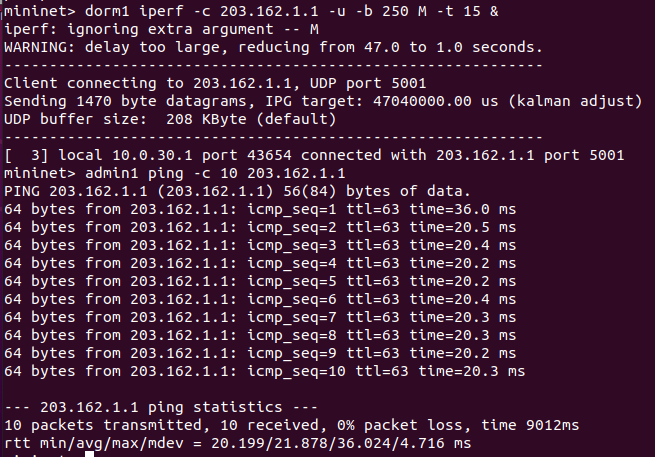
\includegraphics[width=0.8\linewidth]{image/ping_test2_m2.png}
    \caption{Tỷ lệ rớt gói của Admin khi WAN nghẽn trong mạng 3 lớp}
    \label{fig:ping_test2_m2}
\end{figure}